\newpage

\section{Integración}

Gracias a la selección de los componentes, los cálculos realizados, y el diseño de los distintos componentes, fue posible el diseñar y buscar los modelos de los distintos componentes para la simulación total de nuestro sistema compostador.

Para realizar este modelo CAD, primero se procedió a utilizar la estructura como pieza fija, y en relación a ella colocar los demás componentes que constituyen el sistema.

Al tener la estructura como pieza central y referencia, se procedió a armar los distintos subsistemas, antes de fijarlos en la estructura.

Como primer punto se colocó el sistema de calefacción, el cual va colocado en las esquinas del soporte central, este sistema a su vez nos ayudó a mantener en su lugar en contenedor, después de colocar el contenedor en su lugar se procedió a introducir el eje de aireación por las aberturas en los extremos del contenedor

Después de introducir el eje, este es colocado en sus rodamientos de soporte fijados en la estructura principal, de tal forma que se mantienen alineados con respecto al eje, con el eje montado es posible colocar las palas de agitación en el interior del contenedor, accesando al interior del contenedor por la compuerta superior que permite la extracción del compost.

En la lateral izquierda del contenedor se montan los ventiladores de ingreso y extracción del flujo de aire, el ventilador de extracción a su vez esta recubierto con el sistema de escape, en forma de chimenea, que en el interior con tiene el filtro de carbón encargado de eliminar los malos olores.

En el extremo contrario de contenedor, el eje de aireación sobresale sobre su rodamiento para permitir el montaje de la polea conducida,conectada mediante una banda a la polea motriz que esta conectada al eje motriz del motor-reductor, este a su vez esta montado sobre una placa de acero que permite un leve desplazamiento para tensar la banda y pueda hacer buena transmisión de movimiento.

En la parte superior de ese lado de la estructura, gracias a la ayuda de otra placa de acero, se coloca el triturador de materia orgánica, colocando el triturador hasta el otro extremo para tener la libertad de girar la palanca encargada de trasmitir el movimiento al eje triturador.

De la salida del triturador se coloca un conducto que nos permita el llevar la materia orgánica ya triturada el interior del contenedor.

En la parte inferior de la estructura se coloca el recipiente de agua, del cual mediante la ayuda de una bomba se tomará el liquido cuando sea necesario elevar la humedad de la materia orgánica.

En la parte superior de la estructura interfaz del usuario, la cual proporciona la información de las condiciones de operación del sistema completo.

\newpage
\begin{figure}[h]
    \centering
        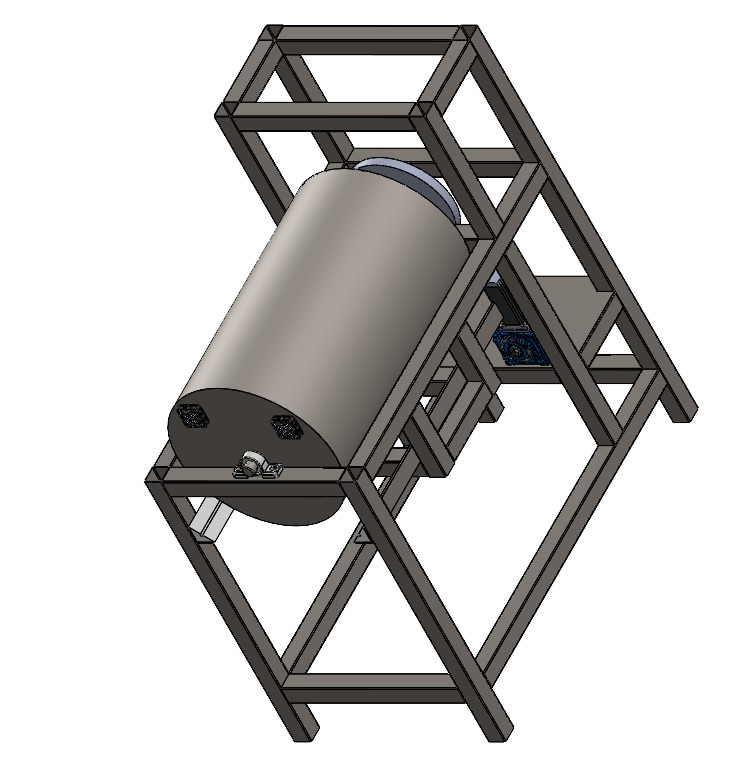
\includegraphics[scale=0.55]{images/Capitulo 4/Ensambe total.jpeg}
        \caption{Integración final del sistema de compostaje}
    \label{fg:EF}
\end{figure}


En la imagen anterior,(figura \ref{fg:EF}), se puede observar la totalidad de los sistemas integrados, este modelo es el que se buscará implementar de manera física.